\let\negmedspace\undefined
\let\negthickspace\undefined
\documentclass[journal]{IEEEtran}
\usepackage[a5paper, margin=10mm, onecolumn]{geometry}
%\usepackage{lmodern} % Ensure lmodern is loaded for pdflatex
\usepackage{tfrupee} % Include tfrupee package

\setlength{\headheight}{1cm} % Set the height of the header box
\setlength{\headsep}{0mm}     % Set the distance between the header box and the top of the text

\usepackage{gvv-book}
\usepackage{gvv}
\usepackage{cite}
\usepackage{amsmath,amssymb,amsfonts,amsthm}
\usepackage{algorithmic}
\usepackage{graphicx}
\usepackage{textcomp}
\usepackage{xcolor}
\usepackage{txfonts}
\usepackage{listings}
\usepackage{enumitem}
\usepackage{mathtools}
\usepackage{gensymb}
\usepackage{comment}
\usepackage[breaklinks=true]{hyperref}
\usepackage{tkz-euclide} 
\usepackage{listings}
% \usepackage{gvv}                                        
\def\inputGnumericTable{}                                 
\usepackage[latin1]{inputenc}                                
\usepackage{color}                                            
\usepackage{array}                                            
\usepackage{longtable}                                       
\usepackage{calc}                                             
\usepackage{multirow}                                         
\usepackage{hhline}                                           
\usepackage{ifthen}                                           
\usepackage{lscape}
\begin{document}

\bibliographystyle{IEEEtran}
\vspace{3cm}

\title{4.5.8}
\author{EE25BTECH11006 - ADUDOTLA SRIVIDYA}
% \maketitle
% \newpage
% \bigskip
{\let\newpage\relax\maketitle}

\renewcommand{\thefigure}{\theenumi}
\renewcommand{\thetable}{\theenumi}
\setlength{\intextsep}{10pt}

\textbf{Question}: The value of $\lambda$ for which the vectors $3i-6j+k$ and $2i-4j+\lambda k$ are parallel is\\
a) $2/3$ \quad
b) $3/2$ \quad
c) $5/2$ \quad
d) $2/5$ \quad

\textbf{Solution:}\\
Given,
\begin{align}
    \myvec{2\\-4\\ \lambda } \text{ is parallel to }  \myvec{3\\-6\\1}
\end{align}

If the vectors are parallel, then they are linearly dependent. Hence,
\begin{align}
    \myvec{3 & 2 \\ -6 & -4 \\ 1 & \lambda}\vec{x} = \myvec{0 \\ 0 \\ 0}
\end{align}

\begin{align}
\myvec{3 & 2 \\ -6 & -4 \\ 1 & \lambda}
\xrightarrow{R_1 \rightarrow \tfrac{R_1}{3}}
\myvec{1 & \tfrac{2}{3} \\ -6 & -4 \\ 1 & \lambda}
\xrightarrow{R_2 \rightarrow R_2 + 6R_1}
\myvec{1 & \tfrac{2}{3} \\ 0 & 0 \\ 1 & \lambda}
\xrightarrow{R_3 \rightarrow R_3 - R_1}
\myvec{1 & \tfrac{2}{3} \\ 0 & 0 \\ 0 & \lambda - \tfrac{2}{3}}
\end{align}

Swap $R_2$ and $R_3$
\begin{align}
    \myvec{1 & \tfrac{2}{3} \\ 0 & \lambda - \tfrac{2}{3} \\ 0 & 0}
\end{align}

Gauss-Jordan elimination depending on \(\lambda\): \\


\textbf{If} \(\lambda = \tfrac{2}{3}.\) \\
Then $R_2$ becomes zero and we have
\begin{align}
    \myvec{1 & \tfrac{2}{3} \\ 0 & 0 \\ 0 & 0}
\end{align}
 Rank = 1 \(\Rightarrow\) columns dependent \(\Rightarrow\) vectors parallel.
 Therefore,
 \begin{align}
     \lambda = \dfrac{2}{3}
 \end{align}


\newpage
\begin{figure}[H]
    \centering
    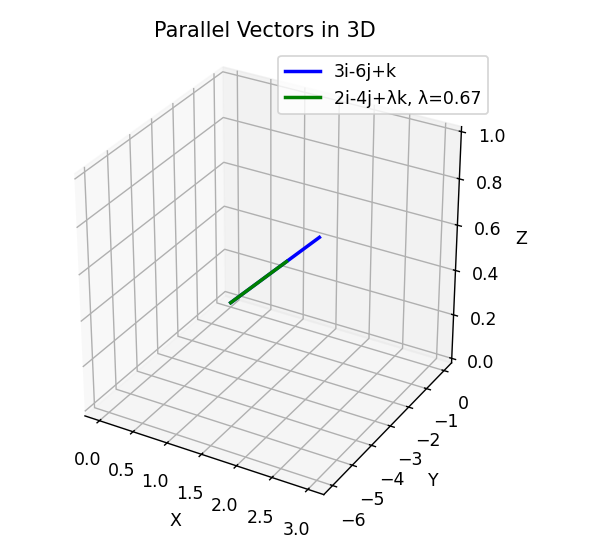
\includegraphics[width=0.7\columnwidth]{figs/fig.png}
    \caption{Vectors $3i-6j+k$ and $2i-4j+\lambda k$ (parallel in 3D)}
    \label{fig:Vectors}
\end{figure}

\end{document}